
\clearemptydoublepage
\pagestyle{empty}\thispagestyle{empty}

\vspace*{\fill}

\section*{Les auteurs}


Ce livre est issu du mooc \emph{Scratch au collège} diffusé au printemps 2017 par une équipe formée de :
\begin{center}
Arnaud Bodin\\
Loïc Arsicaud\\
Nathalie Bernard\\
François Recher
\end{center}

\bigskip 


Les activités Scratch ont été écrites par Arnaud Bodin et validées par l'équipe. 
Nous avons utilisé la version 2 de Scratch, il peut y avoir des variations 
d'une version à l'autre, même si les principes généraux restent les mêmes. 
Les vidéos sont accessibles depuis la chaîne \emph{Youtube} :\\
\centerline{
\href{https://www.youtube.com/c/ScratchAuCollege}{youtube.com/ScratchAuCollege}}


\bigskip 

Les activités débranchées ont été écrites par Arnaud Bodin et relues par Stéphanie Bodin et François Recher.

\bigskip 

L'idée de faire une feuille sur le thème \og{}diviser pour régner\fg{} fait suite à une discussion avec Martin Quinson sur son \og{}crêpier psycho-rigide\fg{}.
Merci à Éric Wegrzynowski pour son idée d'activité sur la distance de Levenshtein ! Enfin, merci à tous les participants du mooc. 

\bigskip 

Nous remercions l'équipe du service multimédia de l'université de Lille 1 pour son travail, en particulier Damien Deltombe pour la réalisation des vidéos, Téodorina Tibar pour l'ingénierie pédagogique et Yannick Bonnaz pour le graphisme.


\bigskip 

Ce projet est porté par le site Exo7 et l'IREM de Lille. 
Nous avons bénéficié du soutien de l'université de Lille 1, de la COMUE Lille Nord de France et d'une bourse Google CS4HS (\emph{Computer Science for High School}).

\bigskip 

\begin{center}
\LogoExoSept{2}\qquad\qquad\qquad
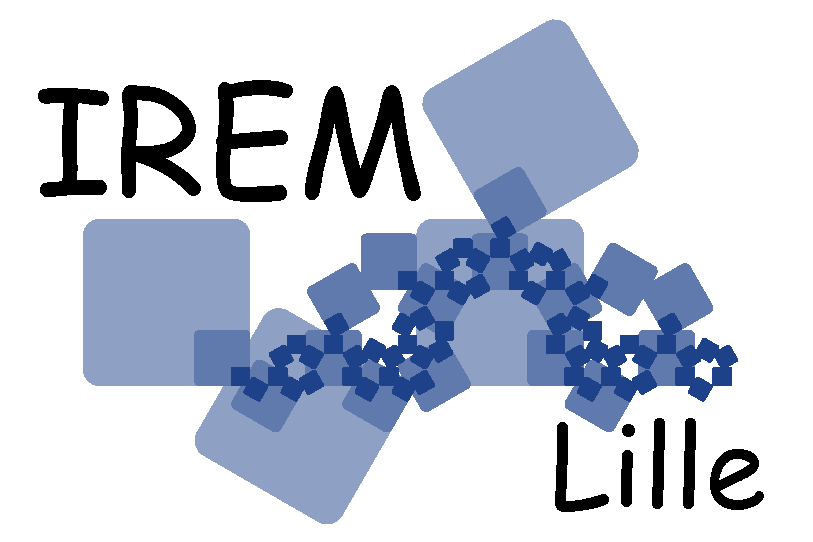
\includegraphics[scale=0.2]{../divers/logo_IREM_de_Lille.pdf}
%\includegraphics[scale=0.2]{../divers/logo_irem_entete.png}
\end{center}


\begin{center}

\includegraphics[scale=0.15]{../divers/logo-lille1-2014.pdf}\qquad
%
\includegraphics[scale=0.15]{../divers/Logo-Univ-Lille-1-new.png}\qquad
\raisebox{3pt}{
\includegraphics[scale=0.25]{../divers/logo-comue.png}}\qquad\qquad

\includegraphics[scale=0.1]{../divers/logo-google.jpg}
\end{center}



\vspace*{\fill}


\begin{center}
Ce livre est diffusé sous la licence \emph{Creative Commons -- BY-NC-SA -- 3.0 FR}.


Sur le site Exo7 vous pouvez télécharger gratuitement le livre en couleur\\
et aussi récupérer les fichiers sources.

\end{center}




%\pagenumbering{gobble} % remove page numbering 
%\printindex
%\pagenumbering{arabic}

